\chapter{Controllo}

Il problema del controllo del moto di un manipolatore consiste nella \textbf{determinazione} dell’andamento temporale delle coppie generalizzate (\textbf{generalized torque)}, che gli attuatori devono applicare ai giunti \textbf{affinché venga eseguito il compito assegnato}, rispettando specifiche sul transitorio e sul comportamento in regime permanente.

Lo schema di controllo può essere sviluppato:
\begin{enumerate}
	\item Nello \textbf{spazio dei giunti}
	\item Nello \textbf{spazio operazionale}
\end{enumerate}

tenendo conto che la descrizione del compito è solitamente elaborata nello spazio operazionale, mentre le azioni di controllo esercitate dagli attuatori sono definite nello spazio dei giunti.\\

\subsubsection{Joint space control}
\begin{figure}[!ht]
	\centering
	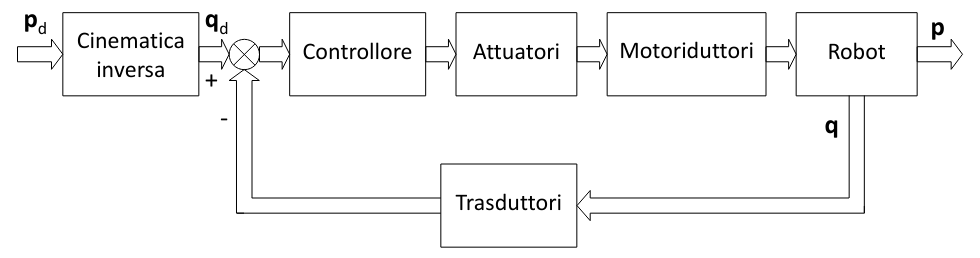
\includegraphics[width=0.7\linewidth]{images/joint_control_1}
	\caption{Schema generale di \textit{joint space control}}
	\label{fig:jointcontrol1}
\end{figure}

L’azione di controllo fa sì che $q(t)$ insegua il vettore $q_d(t)$ della traiettoria desiderata ai giunti, ricavato dalla cinematica inversa (che è comodamente disaccoppiata dal controllo).

\textbf{Svantaggio}: Non si ha nè un feedback, nè un controllo diretto sulla variabile dello spazio operazionale $\mathbf{p}$ $\implies$ dobbiamo avere una cinematica inversa perfetta (ma tolleranze di costruzione, elasticità ai giunti, giochi nei motoriduttori potrebbero causare imprecisioni nella posa della punta operativa).\\



\subsubsection{Operational space control}
\begin{figure}[ht!]
	\centering
	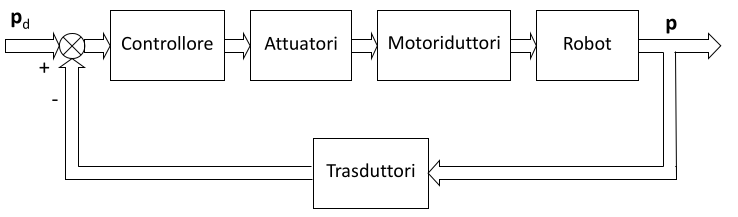
\includegraphics[width=0.7\linewidth]{images/operational_control_1}
	\caption{Schema generale di \textit{operational space control}}
	\label{fig:operationalcontrol1}
\end{figure}

Qui cerchiamo di fare inseguire un vettore $\mathbf{p}_d$ definito nello spazio operazionale. Con questa tecnica introduciamo una \textbf{complessità maggiore}, visto che la cinematica inversa è ora inclusa nel controllore. Il \textbf{vantaggio} però è quello di poter operare direttamente nello spazio operazionale.\\
Anche se in primo luogo potrebbe non sembrare un vantaggio (la “misura” di $\mathbf{p}$ è spesso ricavata indirettamente da misure ai giunti per mezzo della cinematica diretta $\implies$ sembra come se si "ritorni" allo stesso svantaggio di imprecisione della cinematica inversa che c'era nel controllo sui giunti): questo controllo è però utile (ad esempio) come base per il controllo dell’interazione con l’ambiente.\\

\subsubsection{Cosa vedremo}
Vedremo che la presenza di \textbf{motoriduttori} con elevato rapporto di trasformazione tende a \textbf{linearizzare la dinamica} del manipolatore e quindi a disaccoppiare i giunti, grazie alla riduzione degli effetti non lineari $\implies$ si giustifica in tal caso l’adozione di una strategia di \textbf{controllo decentralizzato}, a giunti indipendenti. 

Questo però introduce uno svantaggio: i motoriduttori introducono possibili fenomeni di elasticità, gioco ed attriti non lineari, talora più "fastidiosi" degli effetti di accoppiamento fra i giunti. L’utilizzo di \textbf{motori ad azione diretta} elimina questi problemi ma mantiene rilevanti gli effetti non lineari e di accoppiamento fra i giunti, che non possono essere trascurati o considerati come disturbi $\implies$ diventa opportuno in tal caso utilizzare una strategia di \textbf{controllo centralizzato}, che tenga conto della dinamica non lineare del manipolatore. Svantaggio: la legge di controllo è necessariamente non lineare e computazionalmente pesante.





\section{Attuatori elettrici}
Prima di introdurre i sistemi di controllo, iniziamo parlando di come poter modellare gli attuatori elettrici che andremmo ad utilizzare.

Gli attuatori maggiormente impiegati sono motori elettrici in corrente continua comandati in armatura, corredati di un amplificatore di potenza e di un eventuale anello di retroazione della corrente di armatura: a seconda delle caratteristiche del regolatore inserito, il comportamento dell’attuatore può essere assimilato:
\begin{itemize}
	\item Ad un generatore di velocità controllata (\textbf{velocity controlled})
	\item Ad un generatore di coppia controllata (\textbf{torque controlled})
\end{itemize}

In fig. \ref{fig:electricactuator1} possiamo vedere il modello del motore.

\begin{figure}[th!]
	\centering
	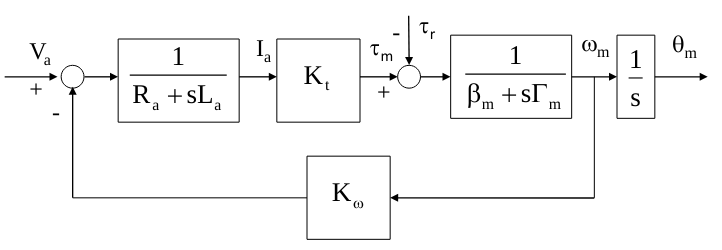
\includegraphics[width=0.7\linewidth]{images/electric_actuator_1}
	\caption{Modello del motorore comandato in armatura}
	\label{fig:electricactuator1}
\end{figure}

Dove:
\begin{itemize}
	\item $\omega_m$ e $\theta_m$ sono la velocità e la posizione angolare dell’albero
	motore
	\item $V_a$ e $I_a$ sono la tensione e la corrente del circuito di armatura
	\item $\tau_m$ è la coppia motrice, mentre $\tau_r$ è la coppia dovuta al carico
\end{itemize}


\subsection{Derivazione modello}

Partendo dal modello illustrato in fig. \ref{fig:electricactuatorcircuit}, possiamo derivare il circuito mostrato in fig. \ref{fig:electricactuator1}.

\begin{figure}[th!]
	\centering
	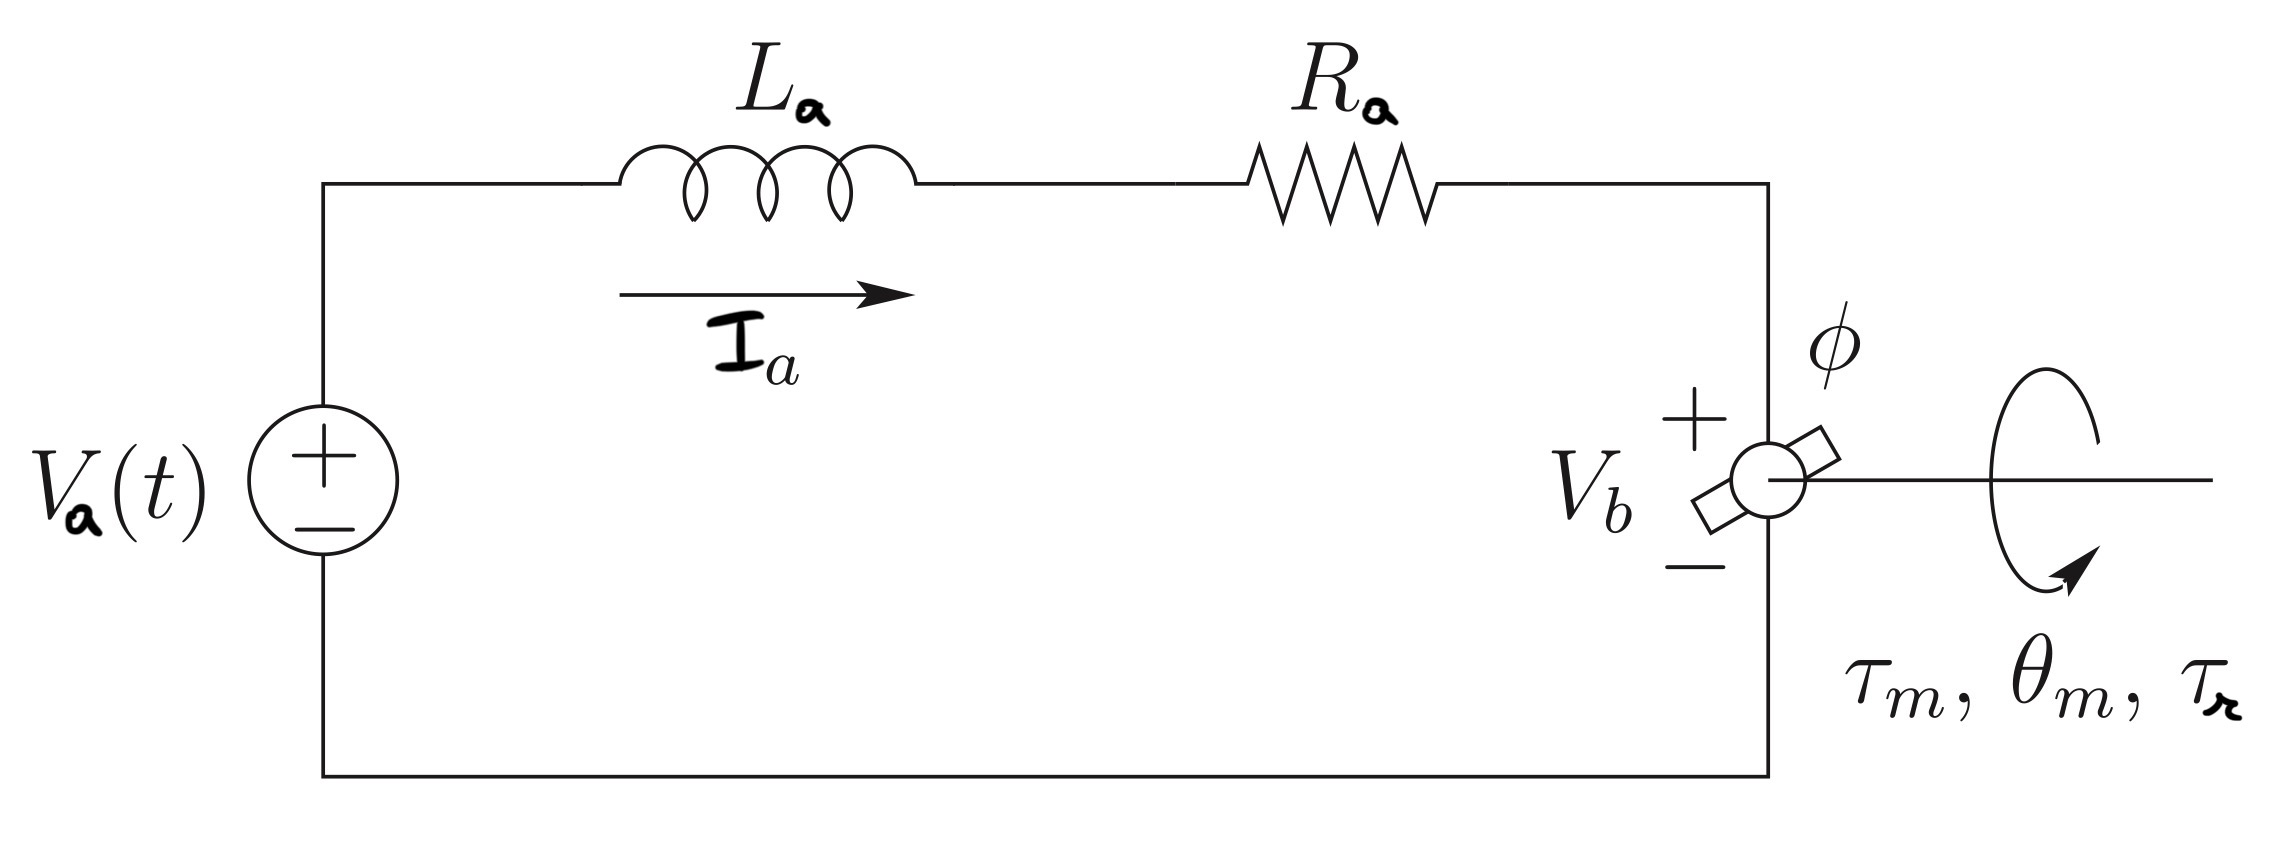
\includegraphics[width=0.7\linewidth]{electric_actuator_circuit.jpg}
	\caption{Modello circuitale del motore}
	\label{fig:electricactuatorcircuit}
\end{figure}

Il bilancio elettrico dell'armatura è definito da:
\begin{align}\label{eq:armature_balance}
L\frac{dI_a}{dt} + RI_a = V_a - V_b
\quad
\xRightarrow{\mathcal {L}}
\quad
\begin{aligned}
V_a &= (R_a + sL_a)I_a + V_g\\
V_g &= K_{\omega} \omega_m
\end{aligned}
\end{align}
Dove $V_g$ è la \textbf{\textit{back-emf}}, ovvero la ogni talvolta che un conduttore si muove in un campo magnetico, ai suoi terminali viene generata una tensione $V_b$ proporzionale alla velocità del conduttore nel campo (cioè proporzionale a $\omega_m$). Questa tensione, chiamata \textit{back-emf}, tenderà ad opporsi al flusso di corrente nel conduttore.

Mentre il bilancio meccanico è definito da:
\begin{align}
\tau_m &= (s\Gamma_m + \beta_m)\omega_m + \tau_r \\
\tau_m &= K_i\Gamma_a
\end{align}
Dove $\Gamma_m$ e $\beta_m$ sono rispettivamente il momento d'inerzia e il coefficiente di attrito viscoso dell'albero motore.

Questo deriva da:
\begin{enumerate}
	\item Ricordando da fisica 1: $F = ma \leftrightsquigarrow \tau = I\alpha$ dove $I$, $\alpha$ sono il momento di inerzia e l'accellerazione angolare
	\item Considerando il motore: $\tau_m = \Gamma_m\dot{\omega}_m$
	\item Ora aggiungiamo l'attrito viscoso (che come ricordiamo è proporzionale alla velocità): $\tau_m - \beta_m\omega_m = \Gamma_m\dot{\omega}_m$
	\item Passiamo a Laplace: $\tau_m = \beta_m\omega_m + \Gamma_m s\omega_m \implies \tau_m = (s\Gamma_m + \beta_m)\omega_m \quad \square$ 
\end{enumerate}


\subsection{Amplificatore di potenza}
Visto che solitamente $V_a$ ha valori elevati, si tende ad utilizzare un \textbf{amplificatore di potenza} per poter comandare il motore con una tensione $V_c \ll V_a$: il nuovo circuito è illustrato in fig. \ref{fig:electricactuator2}. 

$G_v$ è il guadagno di tensione, mentre $T_v$ è una costante di tempo trascurabile (poiché nell’ordine di 10-100 kHz), di conseguenza il blocco dell’amplificatore di potenza può essere assimilato al solo guadagno $G_v$.


\begin{figure}[th!]
	\centering
	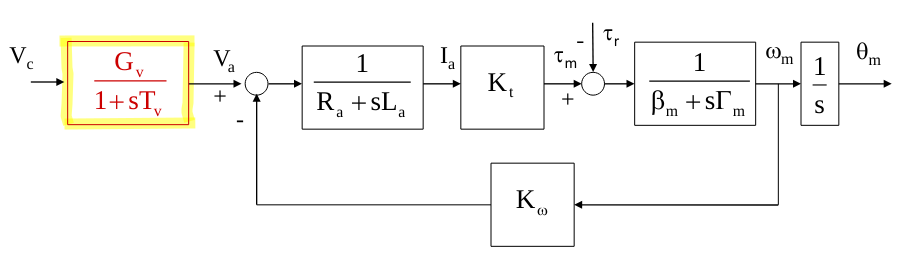
\includegraphics[width=0.7\linewidth]{images/electric_actuator_2}
	\caption{Modello motore con amplificatore di potenza}
	\label{fig:electricactuator2}
\end{figure}



\subsection{Torque generator}

Possiamo ora completare il circuito aggiungendo una retroazione sulla corrente $I_a$ e un compensatore che utilizzi tale feedback. Questo è illustrato in fig. \ref{fig:electricactuator3}.

\begin{figure}[th!]
	\centering
	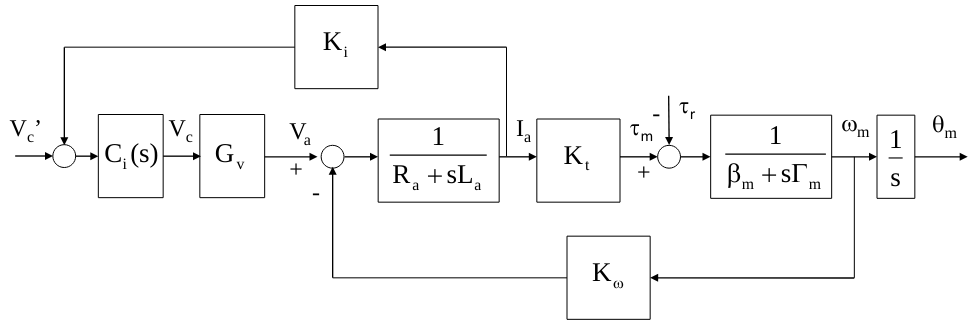
\includegraphics[width=0.7\linewidth]{images/electric_actuator_3}
	\caption{Circuito motore in modalità torque generator}
	\label{fig:electricactuator3}
\end{figure}

In questa modalità, come accennato, il motore si comporta come un \textit{torque-controlled generator}. Questo perchè, con $K_i \neq 0$, se si sceglie $K_i \gg R_a$ otteniamo il seguente steady-state:
$$
\tau_m \approx \frac{K_t}{K_i}(V^{'}_c - \frac{K_\omega}{G_v}\omega_m)
\approx
\frac{K_t}{K_i}V^{'}_c
$$
(supponendo $G_v \gg 1 \implies \frac{K_\omega}{G_v} \to 0$). Questo significa che possiamo impostare il torque del motore giocando sul voltaggio di controllo $V^{'}_c$, che sarà dipendente solo da quest'ultimo (e non, e.g., dalla velocità angolare).




\subsection{Velocity generator}

Se invece rimuoviamo il feedback di corrente, ovvero $K_i = 0$, possiamo vedere come sia possibile impostare a piacimento la velocità del motore (invece della coppia come in precedenza).

\begin{figure}[th!]
	\centering
	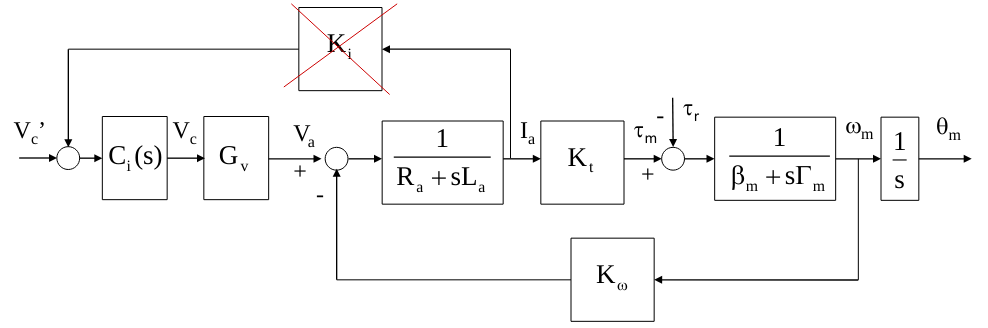
\includegraphics[width=0.7\linewidth]{images/electric_actuator_4}
	\caption{Circuito motore in modalità velocity generator}
	\label{fig:electricactuator4}
\end{figure}

Analizzando questo caso, ricordandoci che il coefficiente di atttrito viscoso meccanico $\beta_m$ è trascurabile rispetto al coefficiente di attrito viscoso elettrico:
$$
\beta_m \ll \frac{K_\omega K_t}{R_a}
$$
Supponendo $C_i(s) = 1$ e $\tau_r = 0$, otteniamo:
$$
\omega_m \approx \frac{G_v}{K_\omega}V^{'}_c
$$

Ovvero, in questo caso, possiamo impostare la velocità angolare a piacere.



\subsection{Torque generator \textit{vs.} Velocity generator}


Quando ci conviene utilizzare uno invece che l'altro?
In seguito vedremo che in tutte le applicazioni in cui è necessario ottenere un’elevata reiezione di coppie di disturbo, come nel caso del \textbf{controllo decentralizzato a giunti indipendenti}, è opportuno NON inserire l’anello di controllo in corrente ed utilizzare i motori come \textbf{generatori di velocità}.

Al contrario, in caso di strategie di \textbf{controllo centralizzate}, è consigliabile introdurre l’anello di retroazione in corrente ed utilizzare i motori come \textbf{generatori di coppie} (opportuni accorgimenti vengono adottati in entrambi i casi per limitare la corrente ed evitare danni ai dispositivi).

E' possibile vedere questa differenza calcolando le relazioni input/output fra $\omega_m$ e $V^{'}_c$, $\tau_r$. Da queste equazioni si può vedere che senza feedback di corrente (i.e. velocity-controlled generator) si ha una reiezione migliore della coppia di disturbo $\tau_r$: i coefficienti legati a $\tau_r$ in questo caso sono molto minori del caso torque-controlled ($\implies$ riduciamo di più gli effetti dei disturbi).

Semplificando:
\begin{align}
\omega_m^{\text{velocity}} &= \alpha_{\text{velocity}} V^{'}_c + \lambda_{\text{velocity}}\tau_r \\
\omega_m^{\text{torque}} &= \alpha_{\text{torque}} V^{'}_c + \lambda_{\text{torque}}\tau_r
\end{align}

se il primo è per il caso velocity-controlled, mentre il secondo per il caso torque-controlled abbiamo che $\lambda_{\text{velocity}} \ll \lambda_{\text{torque}}$.







\section{Trasmissions {\small \textit{aka}} motoriduttori}
Vediamo ora in dettaglio gli effetti che i motoriduttori utilizzati nel motore hanno sul sistema.

\begin{figure}[th!]
	\centering
	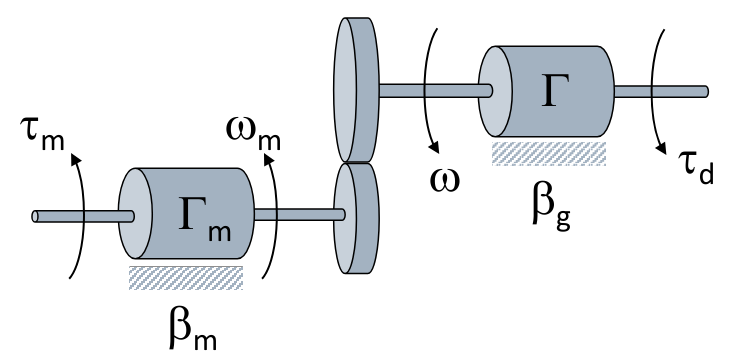
\includegraphics[width=0.5\linewidth]{images/trasmission_1}
	\caption{Motoriduttore}
	\label{fig:trasmission1}
\end{figure}


In generale, se indichiamo con $k_r$ il rapporto di trasformazione (\textit{gear-ratio}) di un motoriduttore ideale, abbiamo che:
$$
\theta_m = k_r\theta
$$
ove $\theta_m$ è la posizione angolare dell’albero motore e $\theta$ è la posizione angolare sul secondario (giunto). Dove $k_r$ è definito come il rapporto fra i due \textit{gears}:
$$
k_r = \frac{r}{r_m} = \frac{\theta_m}{\theta} = \frac{\omega_m}{\omega}
$$

Considerando attriti viscosi e coppie, possiamo scrivere le equazioni di equilibrio:

$$
\begin{array}{l c r}
	{\tau_{_\mathrm{m}}=\Gamma_{_\mathrm{m}}\dot{\omega}_{\mathrm{m}}+\beta_{_\mathrm{m}}\omega_{\mathrm{m}}+\mathrm{fr}_{_{\mathrm{m}}}}\\ {\mathrm{fr}=\Gamma\dot{\omega}+\beta_{_\mathrm{g}}\omega+\tau_{\mathrm{d}}}
\end{array}
$$

(La forza $f$ scambiata tra i due ingranaggi genera una coppia di reazione $fr_m$ per il moto all'asse del motore ed una coppia motrice $fr$ per il moto di rotazione del carico).\\
Dopo alcuni passaggi si ottiene:

$$
\tau_m = \left( \Gamma_m + \frac{\Gamma}{k_r^2} \right) \dot{\omega}_n
+
\left( \beta_m + \frac{\beta_g}{k_r^2} \right)\omega_m
+
\frac{\tau_d}{k_r}
$$

Notiamo che qualunque coppia applicata sul secondario è riportata sul primario ridotta del fattore $k_r$ (e viceversa). \\
Poiché $\mathbf{k_r}$ \textbf{è elevato}, l’effetto di coppie di \textbf{disturbo} agenti sul secondario risulta \textbf{fortemente ridotto} sul primario. Se tali coppie dipendono non-linearmente da $\theta$, allora la presenza di un alto fattore di riduzione tende a \textbf{linearizzare il sistema}.

Nel caso vettoriale (molteplici giunti), possiamo riscrivere alcune utili relazioni:

\begin{align}
	\mathbf{q}_m = \mathbf{K}_r\mathbf{q} \label{eq:trasmission_reduction}\\\
	\boldsymbol{\tau}_m = \mathbf{K}_r^{-1} \boldsymbol{\tau} \label{eq:trasmission_reduction_torque}
\end{align}

Dove quest'ultima deriva dal fatto che con l'aumentare del \textit{gear-ratio} si diminiusce la velocità angolare ma si aumenta il torque (e viceversa).

\section{Controllo decentralizzato a giunti indipendenti \\ {\small \textit{Decentralized Joint Space Control}}}

Nel controllo decentralizzato a giunti indipendenti \textbf{ogni} singolo \textbf{giunto} attuato è considerato come un \textbf{sottosistema SISO disaccoppiato e indipendente}, descritto da un modello dinamico approssimato. Gli \textbf{effetti di accoppiamento} non-lineari presenti nella dinamica propria del robot sono \textbf{considerati come disturbi}.

Lo schema di controllo complessivo è formato da $n$ controllori (uno per ogni giunto), basati su reti di compensazione classiche, ciascuno agente in modo indipendente dagli altri.\\
Ricordiamo che il nostro obiettivo è quello di far eseguire una sequenza $\mathbf{q}(t)$ in modo che $\mathbf{q}(t) \to \mathbf{q}_d(t)$.\\	


\begin{figure}[th!]
	\centering
	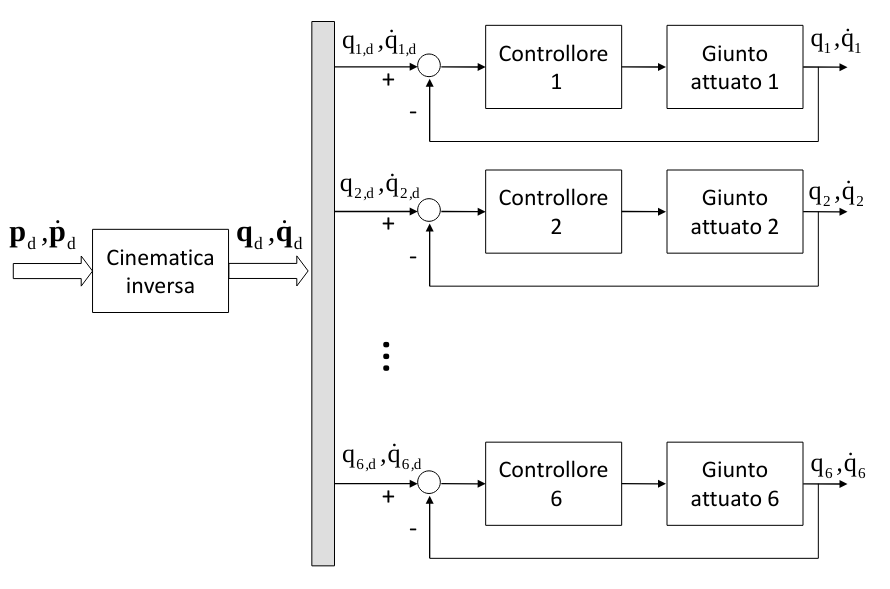
\includegraphics[width=0.7\linewidth]{images/decentralized_joint_space_control_1}
	\caption{Schema generale del controllo a giunti indipendenti}
	\label{fig:decentralizedjointspacecontrol1}
\end{figure}


Come accennato in precedenza, in questo caso andremo a controllare gli attuatori in velocità. È possibile dimostrare (vedi dopo) la seguente assunzione:
$$
\mathbf{G}_v\mathbf{v}_c \approx \mathbf{K}_\omega\mathbf{K}_r\mathbf{\dot{q}}
$$
L'importante di questa espressione è la proporzionalità fra $\mathbf{G}_v$ e  $\dot{\mathbf{q}}$ (velocità), che notiamo essere indipendente dai parametri del manipolatore. Inoltre questa proporzione è tanto più valida quanto velocità/accellerazioni sono piccole (per questa cosa viene in aiuto anche il gear-reduction ratio).

\begin{mdframed}[leftmargin=15pt, rightmargin=15pt, leftline=false, rightline=false]
\textit{Dim.}

\textit{
Partendo dal modello dinamico {\boldmath$B(q)\ddot{q} + C(q, \dot{q})\dot{q} + F_v\dot{q} + g(q) = \tau$} introduciamo in esso la frizione viscosa elettrica. Ovvero poniamo {\boldmath$F_v = F_\text{v. mech.} + F_\text{v. electr.} = F_\text{v. mech.} + K_rK_tR_a^{-1}K_\omega K_r$}. \\
Inoltre dal modello del motore: 
{\boldmath$\tau_m = K_r^{-1} \tau = K_t I_a \implies \tau = K_r K_t I_a$}. Sappiamo anche che $V = Ri \implies i = \frac{V}{R}$ e quindi, ricordando che {\boldmath$V_c = G_v V_c^{'}$}, otteniamo {\boldmath $I_a = R_a^{-1}G_v V_c$}. Unendo il tutto otteniamo {\boldmath $\tau = K_r K_t R_a^{-1}G_v V_c$}.\\
Inserendo tutto nella formula del modello dinamico otteniamo:
\boldmath
$$
B(q)\ddot{q} + C(q, \dot{q})\dot{q} + F_{\text{v. mech.}}\dot{q} + g(q) = K_r K_t R_a^{-1}G_v V_c - K_rK_tR_a^{-1}K_\omega K_r
$$
Ovvero, raccogliendo i termini a destra (ricordando che originalmente quello era $\tau$):
$$
\tau =  K_r K_t R_a^{-1}(G_v V_c - K_\omega K_r \dot{q})
$$
Quello che otteniamo fra le parentesi è l'espressione ipotizzata inizialmente.\\
(la quasi uguaglianza viene dal fatto che $K_r \gg 1$, $R_a$ molto piccolo, $\tau$ non troppo grosso).
}

\raggedleft $\square$
\end{mdframed}


\vspace*{25pt}



Richiamando i capitoli precedenti, ricordiamo che il modello dinamico del manipolatore in assenza di forze scambiate con l’ambiente esterno è espresso da:
\boldmath
\begin{equation}\label{eq:dynamic_no_ext_forces}
B(q)\ddot{q} + C(q, \dot{q})\dot{q} + F_v\dot{q} + g(q) = \tau = K_r \tau_m
\end{equation}
\unboldmath

L'ultima uguaglianza deriva dall'utilizzo dei motoriduttori (vedi (\ref{eq:trasmission_reduction_torque})).

Per elaborare uno schema di controllo decentralizzato ai giunti è opportuno riportare le equazioni dinamiche a monte del motoriduttore (sul primario, i.e. lato motore):
\boldmath
$$
K_r^{-1}B(q)K_r^{-1}\ddot{q}_m + K_r^{-1}C(q, \dot{q})K_r^{-1}\dot{q}_m + K_r^{-1}F_vK_r^{-1}\dot{q} + K_r^{-1}g(q) = \tau_m
$$
\unboldmath

(Questa equazione è ottenuta semplicemente applicando (\ref{eq:trasmission_reduction}) e (\ref{eq:trasmission_reduction_torque}) a (\ref{eq:dynamic_no_ext_forces})).

È possibile notare che $\mathbf{B}(q)$ può essere decomposto in $\mathbf{B}(q) = \bar{\mathbf{B}} + \Delta\mathbf{B}(q)$, ove $\bar{\mathbf{B}}$ è una matrice diagonale costante e $\Delta\mathbf{B}(q)$ è una matrice configuration-dependent. Possiamo quindi riscrivere l'ultima equazione come:
\boldmath
\begin{gather*}
(\bar{B} + \Delta B(q)) K_r^{-1} \ddot{q} + C(q, \dot{q})K_r^{-1}\dot{q} + F_vK_r^{-1}\dot{q} + g(q) = K_r \tau_m \\
\Downarrow \\
K_r^{-1}\bar{B}K_r^{-1}\ddot{q}_m + 
\underbrace{K_r^{-1}\Delta B(q)K_r^{-1}\ddot{q}_m + K_r^{-1}C(q, \dot{q})K_r^{-1}\dot{q}_m + K_r^{-1}g(q)}_{disturbances}
+ K_r^{-1}F_vK_r^{-1}\dot{q}_m  = \tau_m
\end{gather*}


E, come evidenziato nell'equazione, possiamo considerare gli effetti degli altri giunti su quello corrente come \textbf{disturbi}:
\begin{equation}\label{eq:dynamic_disturbances}
	d = K_r^{-1}\Delta B(q)K_r^{-1}\ddot{q}_m + K_r^{-1}C(q, \dot{q})K_r^{-1}\dot{q}_m + K_r^{-1}g(q)
\end{equation}

Inoltre, visto che questi termini sono moltiplicati per $\mathbf{K}_r^{-1}$, \textbf{più alto è il gear-ratio e meno questi termini influenzeranno il nostro sistema} ($d \downarrow$ quando $K_r \uparrow$), portandoci così ad un sistema sempre più lineare e disaccoppiato (ovviamente c'è un limite, visto che gear-ratio altissimi non produrrebbero praticamente alcune velocità).

Riassumendo:


\begin{equation}\label{eq:dynamic_with_disturbances}
K_r^{-1}\bar{B}K_r^{-1}\ddot{q}_m + F_m\dot{q}_m + d = \tau_m
\end{equation}
dove $F_m \triangleq K_r^{-1}F_vK_r^{-1}$. 
\unboldmath



\begin{figure}[t]
	\centering
	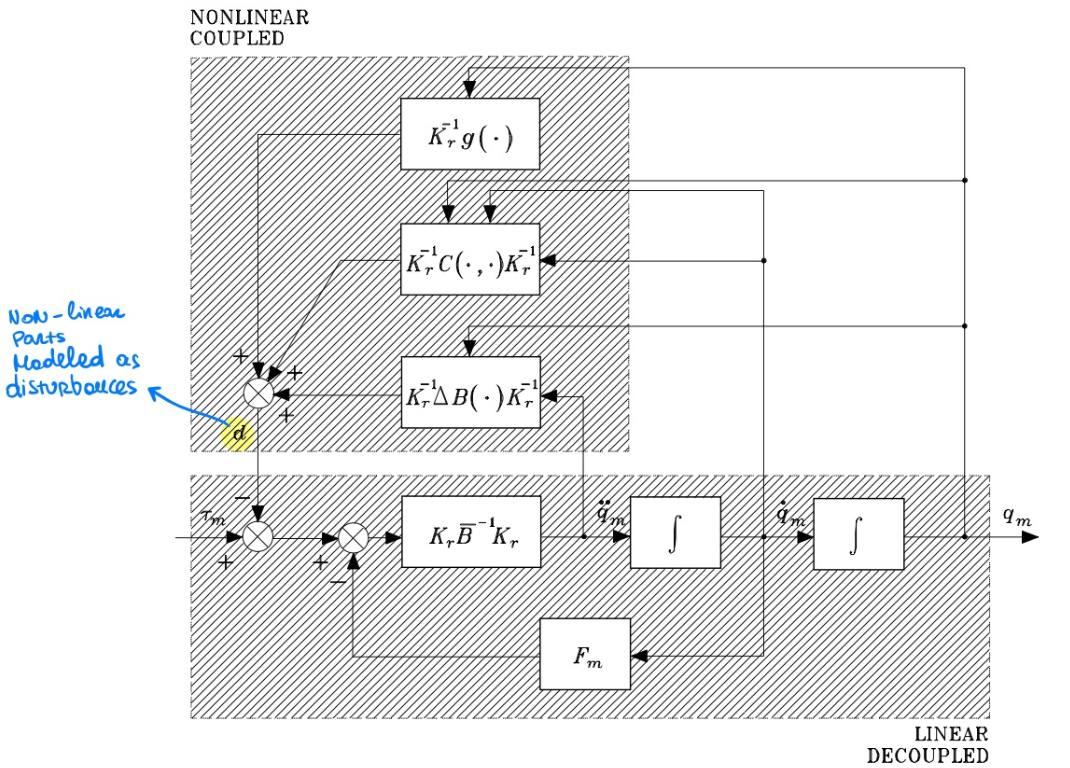
\includegraphics[width=0.7\linewidth]{images/decentralized_joint_space_control_2}
	\caption{Circuito relativo a (\ref{eq:dynamic_with_disturbances})}
	\label{fig:decentralizedjointspacecontrol2}
\end{figure}

Detto questo, per la parte lineare possiamo ora far riferimento alla nota teoria del controllo LTI per sistemi SISO.



\subsection{Controllo del singolo giunto}

Partendo da (\ref{eq:dynamic_with_disturbances}) possiamo estrarre la relazione per un singolo giunto:
\begin{equation}\label{eq:single_joint_dynamic}
\Gamma \ddot{q}_m + \beta \dot{q}_m + d = \tau_m
\end{equation}
dove $\Gamma$ e $\beta$ sono rispettivamente il momento di inerzia totale equivalente ed il coefficiente di attrito viscoso totale equivalente, definiti come segue 
\footnote{notando che ${\mathbf{K}_r}_i^{-1} \alpha {\mathbf{K}_r}_i^{-1} = (1/{\mathbf{K}_r}_i^2) \alpha $}:
$$
\Gamma = \frac{1}{{\mathbf{K}_r}_i^2} \mathbf{\bar{B}}_{ii} 
\quad , \quad
\beta = \frac{1}{{\mathbf{K}_r}_i^2} {\mathbf{F}_m}_i, 
$$

Passando a Laplace (con condizioni iniziali nulle) otteniamo:
\begin{equation}\label{eq:single_joint_dynamic_laplace}
(s\Gamma + \beta) \omega_m(s) = \tau_m(s) - d(s)
\end{equation}
considerando $\omega_n(s)$ come uscita, otteniamo il circuito di fig. \ref{fig:decentralizedjointspacecontrol3} (da notare che questo è equivalente al modello mostrato in fig. \ref{fig:electricactuator4} con $C_i(s) = 1$).

\begin{figure}[th!]
	\centering
	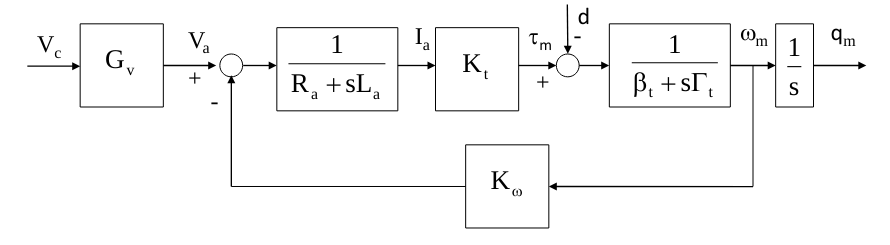
\includegraphics[width=0.7\linewidth]{images/decentralized_joint_space_control_3}
	\caption{Schema a blocchi del singolo giunto}
	\label{fig:decentralizedjointspacecontrol3}
\end{figure}


Cerchiamo ora di semplificare un po' questo modello. Possiamo iniziare supponendo $L_a$ trascurabile, dato che le perdite ad essa associate sono solitamente molto piccole.
Dall'equazione di equilibrio elettrico (\ref{eq:armature_balance}) possiamo quindi rimuovere $L_a$, e ottenere:
$$
V_a - R_aI_a = K_\omega \omega_m
$$
Allora, ricordando che $I_a = \tau_m K_t^{-1}$ e sostituendo $\tau_m$ con l'espressione (\ref{eq:single_joint_dynamic_laplace}) otteniamo 
$$
V_a - R_a K_t^{-1} \tau_m = K_\omega \omega_m
\implies
V_a - R_a K_t^{-1} ((s\Gamma + \beta)\omega_m + d)
= K_\omega \omega_m
$$



Riorganizzando i termini, e ignorando il termine relativo a $\beta$ (visto che è trascurabile rispetto a $\omega_m$), otteniamo:
$$
\left( \frac{R_a \Gamma}{K_t K_\omega}s + 1 \right) \omega_m =
\frac{1}{K_\omega}V_a - \frac{R_a}{K_tK_\omega}d
$$

Da qui possiamo identificare 2 funzioni di trasferimento (a seconda di cosa consideriamo ingresso):

\begin{align}
G_\omega(s) &\triangleq \frac{\omega_m(s)}{V_a(s)} = \frac{1}{K_\omega(1 + sT)} \label{eq:tf_omega} \\
G_d(s) &\triangleq \frac{\omega_m(s)}{d(s)} = -\frac{T}{\Gamma(1 + sT)} = -K_dG_\omega(s)
\end{align}

dove:

$$
T = \frac{R_a \Gamma}{K_t K_\omega} 
\quad , \quad
K_d = \frac{R_a}{K_t}
$$

Da queste equazioni possiamo quindi passare allo schema a blocchi di fig. \ref{fig:decentralizedjointspacecontrol4}.

\begin{figure}[bh!]
	\centering
	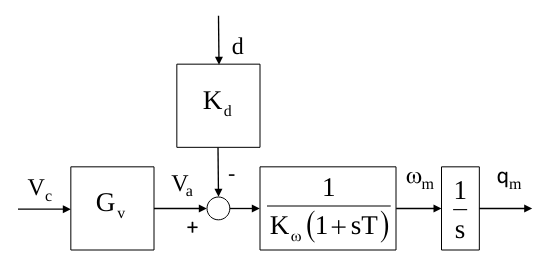
\includegraphics[width=0.6\linewidth]{images/decentralized_joint_space_control_4}
	\caption{Schema a blocchi semplificato}
	\label{fig:decentralizedjointspacecontrol4}
\end{figure}




\vspace*{20pt}
\begin{mdframed}[leftmargin=15pt, rightmargin=15pt, leftline=false, rightline=false]
\subsubsection{Comparazione con le slide di Rizzo}
\textit{Nelle slide è presente il seguente circuito. Anche se a prima vista potrebbe sembrare diverso è in realtà identico a quello di figura \ref{fig:decentralizedjointspacecontrol4}.}

{
	\centering
	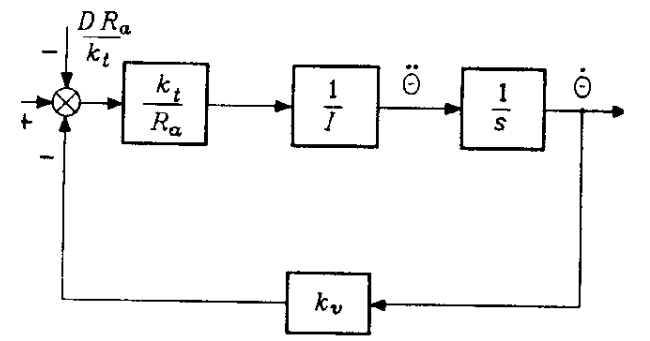
\includegraphics[width=0.6\linewidth]{images/decentralized_joint_space_control_5}
	\label{fig:decentralizedjointspacecontrol5}
	\par
}

\textit{Ricordando la differente notazione: $I \equiv \Gamma$, $k_v \equiv K_\omega$, possiamo unire i 3 blocchi in uno unico. Partiamo dal forward path:}
$$
F(s) = \frac{k_t}{R_a sI}
$$
\textit{Poi, incorporando il feedback, otteniamo}
$$
\frac{F(s)}{1 + F(s)k_v} = 
\frac{ \frac{k_t}{R_a sI} }{1 +  \frac{k_v k_t}{R_a sI} } = \frac{1}{k_v(1 + sT)}
$$

\textit{Ovvero la stessa forma di quanto mostrato in fig. \ref{fig:decentralizedjointspacecontrol4}.}
\end{mdframed}




\vspace{25pt}
\subsection{Struttura del controllo}

In fig. \ref{fig:decentralizedjointspacecontrol6} possiamo vedere lo schema di controllo generale, con retroazione su posizione, velocità e accelerazione (nota: per semplicità $G_v$ è stato incluso nell'anello di controllo più interno).

In generale, il controllore viene progettato modo che si abbia un guadagno elevato nel blocco a monte del punto di ingresso del disturbo (per ottenere un elevato fattore di attenuazione) e in modo che ci sia un’azione integrale, affinché gli effetti della coppia di gravità vengano cancellati in regime permanente.

\begin{figure}[H]
	\centering
	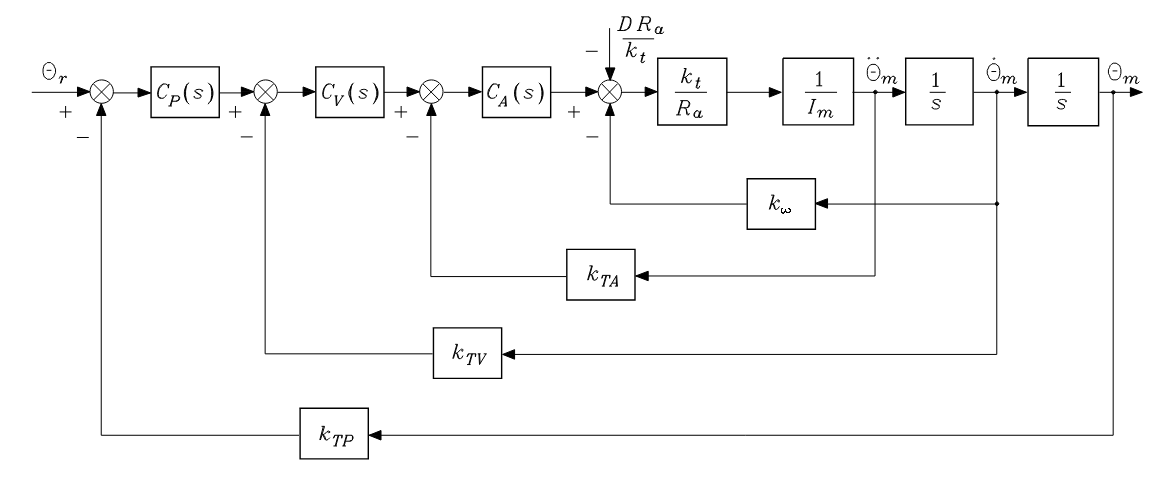
\includegraphics[width=0.9\linewidth]{images/decentralized_joint_space_control_6}
	\caption{Schema generale del controllo}
	\label{fig:decentralizedjointspacecontrol6}
\end{figure}


Queste richieste portano alla scelta di un \textbf{controllore PI (proporzionale-integrale)} della forma:
\begin{equation}\label{eq:pi_controller}
C(s) = K_p \frac{1+sT_p}{s}
\end{equation}






\subsubsection{Retroazione sulla posizione}
Possiamo partire dal caso più semplice, ovvero introducento un controllo con solo la retroazione $k_{TP}$ su $\theta_m$. Poniamo $C_v(s) = C_A(s) = 1$ e $k_{TV} = k_{TA} = 0$, mentre mettiamo $C_p(s)$ nella forma (\ref{eq:pi_controller}).

\begin{figure}[ht!]
	\centering
	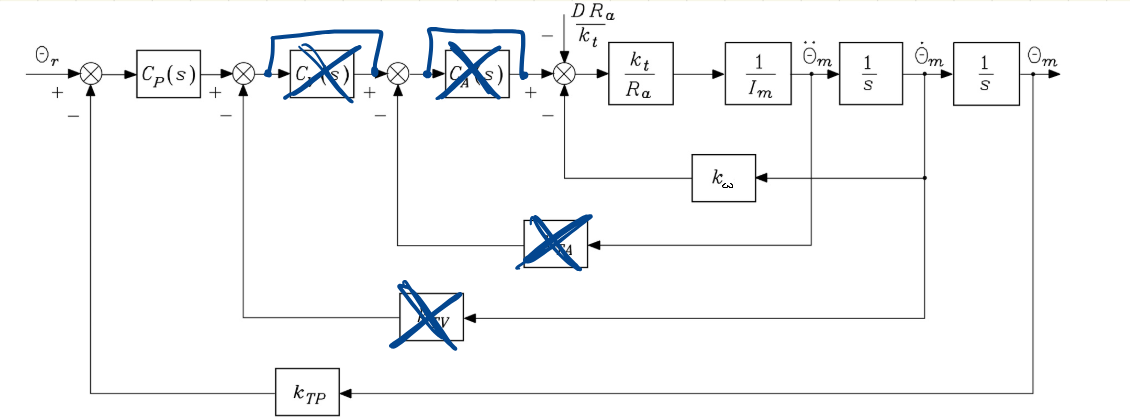
\includegraphics[width=0.7\linewidth]{images/position_feedback}
	\caption{Solo position feedback}
	\label{fig:positionfeedback}
\end{figure}

La funzione di trasferimento del ramo diretto risulta (richiamando (\ref{eq:pi_controller}) e (\ref{eq:tf_omega})):
$$
G(s) = 
\underbrace{C_p(s)}_{(\ref{eq:pi_controller})}
\underbrace{ \frac{1}{K_\omega(1 + sT)} }_{G_\omega(s) =(\ref{eq:tf_omega})}
\frac{1}{s}
= \frac{K_p(1+sT_p)}{s^2K_\omega(1+sT)}
$$
da cui si ricava la funzione di trasferimento ad anello chiuso:
$$
W(s) = \frac{K_p(1+sT_p)}{s^2K_\omega(1+sT) + K_P K_{TP} (1+sT_P)}
$$

Da qui è possibile analizzarne la stabilità, ad esempio tramite il luogo delle radici (vedi fig. \ref{fig:rootlocus1}).

\begin{figure}[ht!]
	\centering
	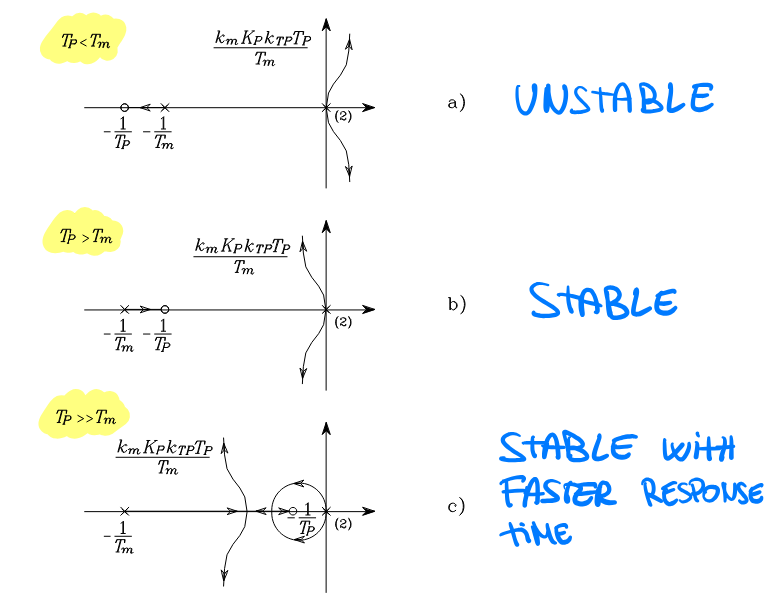
\includegraphics[width=0.7\linewidth]{images/root_locus_1}
	\caption{Root locus per $W(s)$ con solo retroazione sulla posizione}
	\label{fig:rootlocus1}
\end{figure}


I parametri $K_P$ e $T_P$ devono essere scelti in modo da:
\begin{itemize}
	\item Garantire l’asintotica stabilità del sistema in catena chiusa
	\item Evitare oscillazioni significative nella sua risposta
	\item Garantire un elevato fattore di attenuazione del disturbo 
\end{itemize}


Per calcolare meglio i requirements è possibile esprimere $W(s)$ in funzione di $\omega_n$ e $\zeta$:
$$
W(s) = \frac{\frac{1}{K_{TP}}(1+sT_P)}{\left( 1 + \frac{2\zeta}{\omega_n} + \frac{s^2}{\omega_n^2} \right) (1+\tau s) }
$$

Come possiamo vedere anche dal root locus:
\begin{itemize}
	\item Deve essere $T_P > T$ affinché si abbia asintotica stabilità
	\item Se $T_P \gg T$ si velocizza la risposta del sistema (diventano dominanti i poli complessi coniugati). Inoltre per elevati valori del guadagno $K_P$ la pulsazione del polo reale di $W(s)$ tende a quella dello zero ($\tau \approx T_P$) e quindi il sistema risulta rappresentato in prima approssimazione dalla sola dinamica del II° ordine associata ai poli complessi coniugati
	\item La parte reale dei poli dominanti non può comunque essere inferiore a $-1/(2T)$
\end{itemize}

Applicando le regole dell'algebra dei blocchi, è possibile anche ricavare la funzione di trasferimento fra il disturbo $D$ e l’uscita $\theta_m$ del sistema: $\Theta_m(s) / D(s)$.\\
Da questa t.f. è possibile vedere che \textbf{il fattore di attenuazione del disturbo vale} $\mathbf{K_PK_{TP}}$. Valori troppo elevati di $K_P$ possono però portare ad avere oscillazioni inaccettabili sull’uscita (lo smorzamento $\zeta$ risulta troppo piccolo).\\
Il tempo necessario per avere un’attenuazione significativa del disturbo è approssimabile come $T_R = max\{T_P, \frac{1}{\zeta \omega_n}\}$








\vspace{35pt}
\subsubsection{Retroazione di posizione e velocità}

Per questo secondo caso consideriamo il seguente setup (qua $C_A(s)=1$, $k_TA=0$):
$$
C_P(s) = K_P \qquad C_V(s)=K_V\frac{1+sT_V}{s}
$$
Ovvero un'azione solo proporzionale per la posizione, mentre un'azione PI per la velocità.

\begin{figure}[ht!]
	\centering
	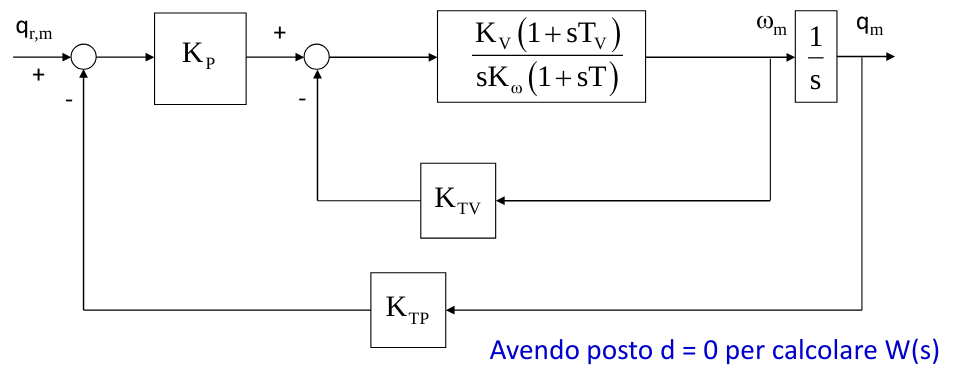
\includegraphics[width=0.7\linewidth]{images/decentralized_joint_space_control_7}
	\caption{Circuito con retroazione su posizione e velocità}
	\label{fig:decentralizedjointspacecontrol7}
\end{figure}


Di nuovo, possiamo analizzare la stabilità del sistema tramite il root-locus della funzione di trasferimento in ciclo chiuso $W(s)$ e gli effetti dei disturbi con la funzione di trasferimento $\Theta_m(s)/D(s)$.
$$
W(s)=\frac{K_P K_V}{K_\omega s^2 + K_V K_{TV} s + K_{TP} K_P K_V}
$$

Saltando nuovamente la forma esplicita di $\Theta_m(s)/D(s)$, possiamo dire che in questo caso il \textbf{fattore di attenuazione del disturbo} è dato dal prodotto $\mathbf{K_P K_{TV} K_V}$, ormai completamente definito, avendo imposto $K_P$ e $K_V$ per imporre i poli desiderati.

Aumentando il guadagno del feedback di posizione $K_P$, è possibile confinare i poli dell'anello chiuso in una regione del piano complesso con grandi valori assoluti della parte reale. Poi, la posizione effettiva può essere stabilita mediante una scelta adeguata di $K_V$.

\begin{figure}[!ht]
	\centering
	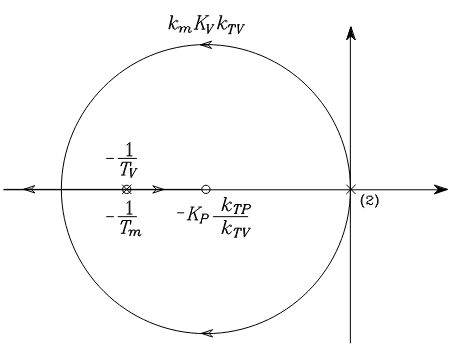
\includegraphics[width=0.5\linewidth]{images/root_locus_2}
	\caption{Root-locus con retroazione di velocità e posizione}
	\label{fig:rootlocus2}
\end{figure}







\vspace{35pt}
\subsubsection{Retroazione di posizione, velocità ed accelerazione}

Per concludere vediamo il controllo con tutti e 3 i feedback:
$$
C_P(s) = K_P \qquad C_V(s)=K_V \qquad C_A(s)=K_A\frac{1+sT_A}{s}
$$

Avendo a disposizione un parametro libero in più, sarebbe
possibile in questo caso:
\begin{itemize}
	\item Assegnare la dinamica desiderata al sistema ad anello chiuso
	\item Imporre il fattore di attenuazione del disturbo
\end{itemize}


\begin{figure}[ht!]
	\centering
	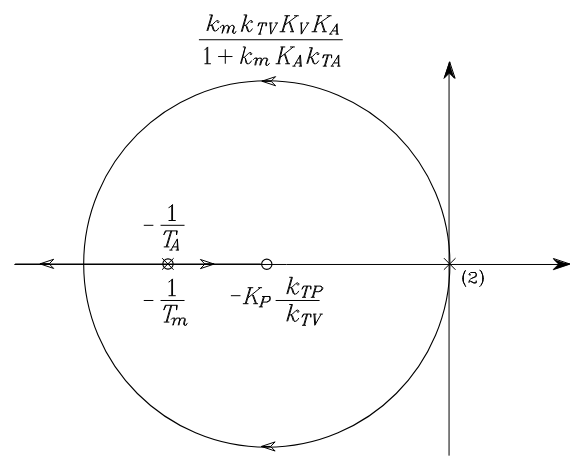
\includegraphics[width=0.5\linewidth]{images/root_locus_3}
	\caption{Root-locus con retroazione di accelerazione, velocità e posizione}
	\label{fig:rootlocus3}
\end{figure}

\textbf{Problema}:
La misura dell’\textbf{accelerazione però non è solitamente disponibile}. Per implementare uno schema di controllo comprendente la retroazione dell’accelerazione risulterebbe necessario ricavarla indirettamente dalle misure disponibili.

Avendo a disposizione la misura diretta della velocità, è possibile \textbf{stimare l’accelerazione} per mezzo di un filtro del primo ordine (vedi fig. \ref{fig:accelerationestimate}), purché avente banda sufficientemente ampia. Scegliendo questa larghezza di banda sufficientemente ampia, gli effetti dovuti ai ritardi di misurazione non sono un problema, e quindi è possibile prendere l'uscita del filtro di accelerazione come quantità per il feedback. Problemi possono comunque incorrere a causa del rumore presente sul segnale di accelerazione così ottenuto.

\begin{figure}[H]
	\centering
	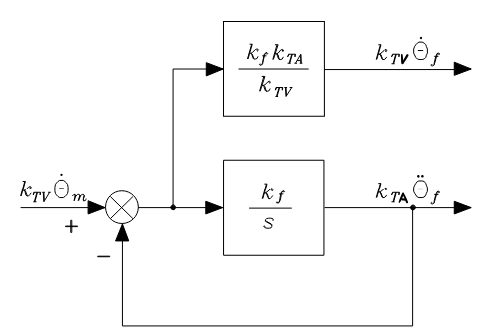
\includegraphics[width=0.4\linewidth]{images/acceleration_estimate}
	\caption{Filtro del I° ordine per la stima dell'accelerazione}
	\label{fig:accelerationestimate}
\end{figure}







\subsection{Attuatori saturanti}
In un’applicazione reale, il comportamento del sistema può allontanarsi da quello del suo modello teorico a causa di dinamiche “parassite” o non lineari, non incluse nella descrizione considerata, con evidenti conseguenze sulle prestazioni del controllo. Una di queste è ad esempio la presenza di attuatori saturanti.

Quest'ultima però può essere modellata semplicemente aggiugendo sul ramo diretto dell’anello di controllo un blocco che rappresenta la seguente relazione:
$$
\begin{cases}
	y_{max} & , \ u(t) > u_{max} \\
	ku(t) & , \ u_{min} \leq u(t) \leq u_{max} \\
	y_{min} & , \ u(t) < u_{min}
\end{cases}
$$


\begin{figure}[H]
	\centering
	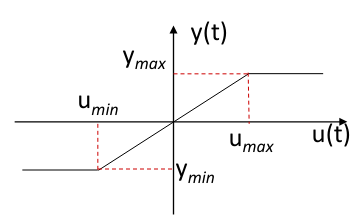
\includegraphics[width=0.4\linewidth]{images/saturation}
	\label{fig:saturation}
\end{figure}


L’inserimento di blocchi di \textbf{saturazione} è solitamente legato a \textbf{necessità di sicurezza e di salvaguardia} del sistema.

Quando le grandezze coinvolte (correnti, tensioni) raggiungono il valore massimo consentito ed entra in azione il blocco di saturazione, l’inseguimento della traiettoria non è più realizzato con le caratteristiche e l’accuratezza prevista. In caso di movimenti PTP non è inusuale che vengano raggiunte situazioni di saturazione: in tal caso infatti è solitamente prioritario raggiungere il più rapidamente possibile la configurazione finale desiderata, anziché rispettare la traiettoria prefissata in ogni istante.







\subsection{Feedforward compensation}
Quando è richiesto l’inseguimento di traiettorie con elevati valori di velocità e di accelerazione, è possibile ridurre l’errore di inseguimento utilizzando i valori del riferimento in velocità (ed in accelerazione) per calcolare termini di compensazione in avanti (feedforward compensation), da sommare all’azione del controllore posto sul ramo diretto.

Si noti che, in generale, calcolare derivate non è possibile (perchè dovremmo "predire il futuro"). In questo caso però essendo la traiettoria nota a priori, non ci sono problemi.

\begin{figure}[H]
	\centering
	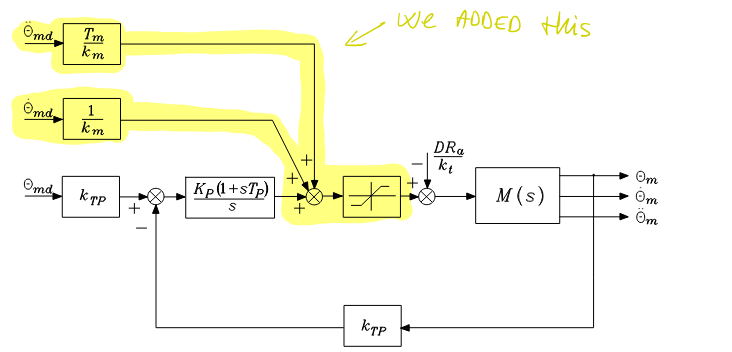
\includegraphics[width=0.7\linewidth]{images/feedforward_compensation}
	\caption{Schema a blocchi del controllo con feedback di posizione e feedforward compensation decentralizzato}
	\label{fig:feedforwardcompensation}
\end{figure}





\subsection{Computed torque	feedworward control}
È possibile aggiungere un altro blocco di feedforward.
Richiamando (\ref{eq:dynamic_with_disturbances}):
\boldmath
$$
K_r^{-1}\bar{B}K_r^{-1}\ddot{q}_m + F_m\dot{q}_m + d = \tau_m
$$
\unboldmath

se vogliamo reiettare perfettamente il disturbo $d$ potremmo provare a calcolarci in anticipo il valore di $d$, per poi sommarlo nel lato destro dell'equazione.

\boldmath
$$
K_r^{-1}\bar{B}K_r^{-1}\ddot{q}_m + F_m\dot{q}_m + \cancel{d} = \tau_m + \cancel{d}
$$
\unboldmath

Ponendo $q\equiv q_d$ ci basta usare (\ref{eq:dynamic_disturbances}) per calcolarci $d$ (offline).
 
\begin{figure}[H]
	\centering
	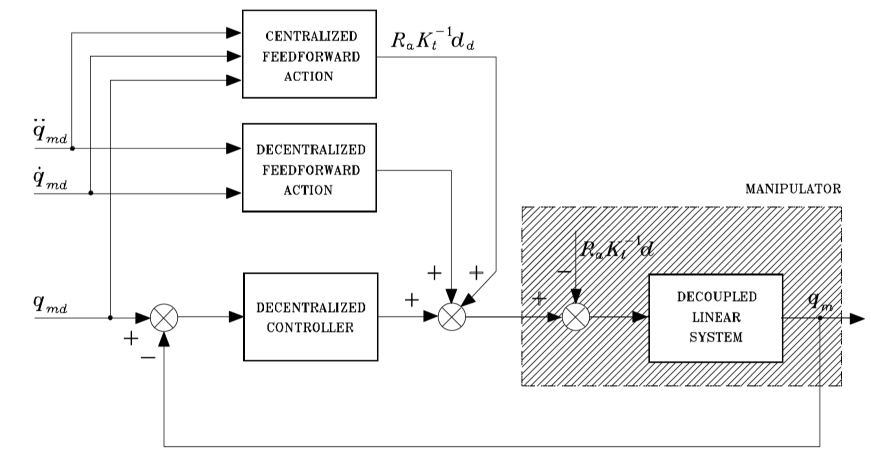
\includegraphics[width=0.7\linewidth]{images/computed_torque}
	\caption{Circuit with computed torque feedworward control}
	\label{fig:computedtorque}
\end{figure}




\section[Controllo centralizzato ai giunti]{Controllo centralizzato ai giunti \\ \small \textit{Centralized Joint Space Control}}

In alcuni casi il \textbf{controllo decentralizzato} a giunti indipendenti \textbf{può risultare inadeguato}. Questo accade, ad esempio, quando:
\begin{itemize}
	\item sono \textbf{richieste velocità operative elevate} $\implies$ le coppie di disturbo strutturato dipendenti dalla velocità (di Coriolis, centrifughe) influiscono pesantemente sul comportamento dei giunti
	\item i \textbf{motori sono ad azione diretta} $\implies$ a causa dell’assenza dei motoriduttori ($\mathbf{K}_r = \mathbf{I}$) non si beneficia di alcuna riduzione degli effetti non lineari e di accoppiamento fra i giunti
\end{itemize}
 
In tali casi gli effetti delle coppie di disturbo $\mathbf{d}$ possono determinare errori troppo elevati di inseguimento della traiettoria.
 
Poiché in questi casi non è possibile ridurre sufficientemente gli effetti indotti dalle coppie di disturbo $\mathbf{d}$, diventa conveniente cercare di eliminare direttamente tali coppie, ricorrendo ad una \textbf{strategia di controllo contenente termini non lineari di compensazione}.\\
Si parla di \textbf{controllo centralizzato} perché la coppia applicata a ciascun giunto risulta funzione anche delle variabili di posizione e velocità degli altri giunti, a differenza di quanto accade nel controllo a giunti indipendenti.
 
Negli schemi di controllo centralizzato il manipolatore è considerato come un \textbf{unico sistema MIMO}, con n ingressi (le coppie applicate ai giunti) e n uscite (le posizioni dei giunti) che interagiscono fra loro secondo relazioni non lineari. La \textbf{legge di controllo} centralizzato dovrà tenere conto del modello dinamico del manipolatore ed essere \textbf{non-lineare} (visto che il modello è non lineare).
 
 
 
\subsubsection{Idea principale}
Il principale approccio di controllo centralizzato è detto a \textbf{dinamica inversa}, perché la coppia di comando è ricavata dall’equazione dinamica del manipolatore a partire dalla conoscenza delle variabili giunto (posizioni e velocità), ovvero dalla risoluzione del problema della dinamica inversa.\\
Ovvero usando il modello dinamico:
\boldmath
$$
B(q)\ddot{q} + C(q, \dot{q})\dot{q} + F_v\dot{q} + g(q) = \tau
$$
\unboldmath

ci calcoliamo $\boldsymbol{\tau}$, che poi andiamo a fornire ai nostri attuatori, che quindi in questo caso saranno in modalità \textbf{torque-controlled}.




\subsubsection{Ora usiamo attuatori torque-controlled}
Come accennato in questo caso abbiamo bisogno di generatori di coppia.

Richiamando la forma semplificata del bilancio elettrico di armatura (\ref{eq:simplified_armature_electrical_balance}), possiamo scrivere:
$$
I_a = R_a^{-a}(V_a - K_\omega \omega_m) = R_a^{-1}(G_vV_c - K_\omega \omega_m)
$$
Dove l'ultima ugualianza deriva dall'amplificatore di potenza: $V_a = G_v V_c$.
Di conseguenza, ricordando (sempre al modello del motore: vedi fig. \ref{fig:electricactuator1}), che $\tau_m = K_t I_a$, possiamo scrivere:
$$
\tau = K_r \tau_m = K_r K_t I_a = K_r K_t R_a^{-1}(G_vV_c - K_\omega \omega_m)
$$
che si può notare essere uguale a (\ref{eq:torque_command}).

Visto che però vogliamo avere un motore torque-controlled (come possiamo ricordare) è necessario inserire la corrente in retroazione. Per magimagia (forse vedi sezione \ref{section:torque_generator}) diciamo che il termine con $K_\omega$ diventa trascurabile e quindi:
$$
I_a = R_a^{-1}(G_vV_c) = G_i V_c
$$
Di conseguenza
\boldmath
$$
\tau = K_r K_t G_i V_c = u
$$
\unboldmath
ove $\mathbf{u}$ è il vettore di comandi disponibili per il controllo.








\subsection{Controllo a dinamica inversa}
L’approccio di controllo a dinamica inversa è basato sull’idea di ottenere una \textbf{linearizzazione della dinamica del sistema per mezzo di una retroazione non lineare} degli stati tale da condurre ad un sistema lineare e disaccoppiato rispetto ad un nuovo vettore di accelerazioni di comando da progettare. Ovvero utilizzamo la tecnica nota come \textbf{feedback linearization}.

Prima di cominciare, per comodità definiamo il modello della dinamica come:
\boldmath
\begin{equation}\label{eq:simplified_notation_dynamic}
B(q)\ddot{q} + n(q, \dot{q}) = \tau = u
\end{equation}
dove:
$$
n(q, \dot{q}) \triangleq C(q, \dot{q})\dot{q} + F_v\dot{q} + g(q)
$$
\unboldmath

Supponendo di poter calcolare esattamente $\mathbf{B(q)}$ e $\mathbf{n(q, \dot{q})}$, definiamo il nostro comando di controllo come
\boldmath
$$
u = B(q)y + n(q, \dot{q})
$$
questo perchè, così facendo, riusciamo ad ottenere una \textbf{linearizzazione esatta del sistema}:
\begin{gather*}
B(q)\ddot{q} + \cancel{n(q, \dot{q})} = \tau = u = B(q)y + \cancel{n(q, \dot{q})} \\
\Updownarrow \\
\cancel{B(q)}\ddot{q} = \cancel{B(q)}y \\
\Updownarrow \\
\ddot{q} = y
\end{gather*}
Il sistema risultante è costituito da n doppi integratori: la i-esima componente $y_i$ del nuovo comando influenza solo il comportamento della i-esima coordinata giunto $q_i$, che risulta indipendente dal moto degli altri giunti.


\begin{figure}[H]
	\centering
	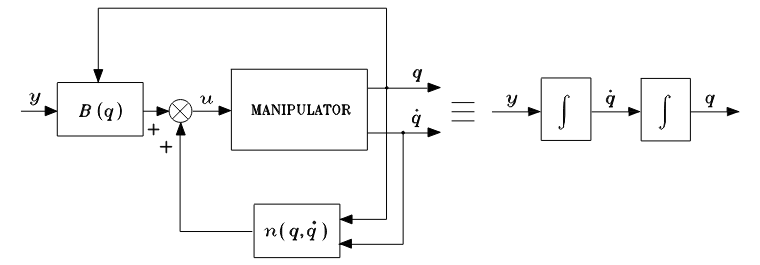
\includegraphics[width=0.8\linewidth]{images/centralized_control_1}
	\caption{Feedback linearization}
	\label{fig:centralizedcontrol1}
\end{figure}

La scelta più semplice per il nuovo comando $\mathbf{y}$ è data da una legge di \textbf{controllo di tipo PD}:
$$
y = -K_P q - K_D \dot{q} + r
$$

che quindi, sostituiendo a $\ddot{q} = y$, otteniamo il seguente sistema di equazioni del secondo ordine:
\begin{equation}\label{eq:2nd_order_dyn_feedback_lin}
\ddot{q} + K_D \dot{q} + K_P q = r
\end{equation}
asintoticamente stabile se le matrici $K_P$ e $K_D$ sono definite positive.
Scegliendo in particolare $K_P$ e $K_D$ diagonali, il sistema rimane disaccoppiato e ad ogni variabile giunto viene assegnata la dinamica corrispondente ai guadagni imposti con:
\unboldmath
$$
\mathbf{K_P} = diag\{\omega_{n1}^2, \ \dots, \ \omega_{nn}^2\}
\quad
\mathbf{K_D} = diag\{2\zeta\omega_{n1}, \ \dots, \ 2\zeta\omega_{nn}^2\}
$$

\boldmath
Il vettore di riferimento $r$ è definito a partire dalla traiettoria desiderata, pianificata ai giunti, come:
$$
r \triangleq \ddot{q}_d + K_D \dot{q}_d + K_P q_d 
$$
Possiamo ora analizzare la dinamica dell'errore di inseguimento, sostituendo la definizione di $r$ a (\ref{eq:2nd_order_dyn_feedback_lin}):
$$
(\ddot{q}_d - \ddot{q}) + K_D(\dot{q}_d - \dot{q}) + K_P(q_d - q) = 0
\implies
\ddot{e} + K_D\dot{e} + K_Pe = 0
$$
se $e(0) = 0$ e $\dot{e}(0) = 0$, l'errore converge a 0 con velocità e caratteristiche determinate da $K_P$ e $K_D$.
\unboldmath

Il sistema risultante è mostrato in fig. \ref{fig:centralizedcontrol2}, dove notiamo due anelli: quello più interno è l'anello di linearizzazione, mentre quello esterno è il controllo (ora lineare) del nostro sistema.

\begin{figure}
	\centering
	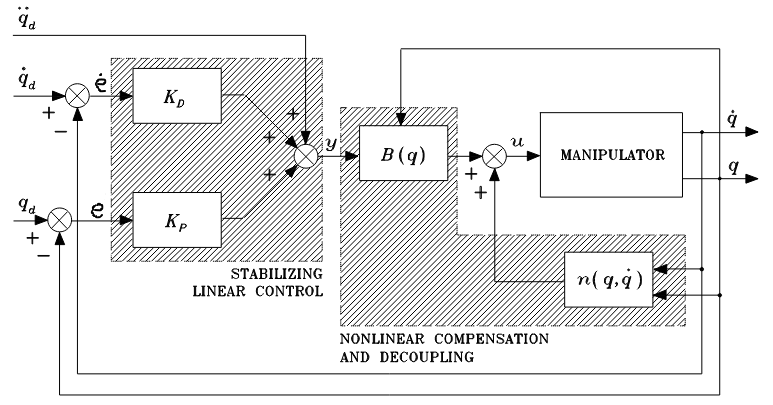
\includegraphics[width=0.7\linewidth]{images/centralized_control_2}
	\caption{Schema a blocchi del controllo a dinamica inversa nello spazio dei giunti}
	\label{fig:centralizedcontrol2}
\end{figure}


\vspace{20pt}
\subsubsection{Problemi}
L’ipotesi di linearizzazione esatta presuppone la capacità di calcolare \textit{online} le matrici $\mathbf{B(q)}$ e $\mathbf{n(q, \dot{q})}$ in modo esatto. Nella pratica però questo non è sempre possibile.
Per compensare a questi errori è necessario utilizzare altre tecniche, ad esempio algoritmi di controllo robusto.

Supponiamo di avere solo delle approssimazioni delle matrici, che chiameremo $\mathbf{\hat{B}(q)}$ e $\mathbf{\hat{n}(q, \dot{q})}$:
\boldmath
\begin{gather*}
B(q)\ddot{q} + n(q, \dot{q}) = \hat{B}(q)y + \hat{n}(q, \dot{q}) \\
\Updownarrow \\
\ddot{q} = B^{-1}\hat{B}y + B^{-1}(\hat{n} - n) \\
\Updownarrow \\
\ddot{q} = y + (B^{-1}\hat{B} - I)y + B^{-1}(\hat{n} - n) \\
\Updownarrow \\
\ddot{q} = y - \eta(q, \dot{q}, y) \\
\Downarrow \\
\ddot{e} + K_D\dot{e} + K_Pe = \eta(q, \dot{q}, y)
\end{gather*}

where
$$
\eta(q, \dot{q}, y) \triangleq (I - B^{-1}\hat{B})y - B^{-1}(\hat{n} - n)
$$

Il sistema ottenuto non è più lineare e disaccoppiato.

Per fortuna, \textbf{nella pratica}, il metodo della dinamica inversa \textbf{risulta abbastanza robusto} anche nel caso di linearizzazione approssimata, per cui viene usato sia senza ulteriori modifiche, sia con l’aggiunta di un termine robustificante.\\

\vspace{10pt}
\subsubsection{Vari schemi visti come dinamica inversa}
Tra gli schemi a dinamica inversa con linearizzazione approssimata, che non prevedono l’inserimento di termini robustificanti, possiamo includere:
\begin{itemize}
	\item \textbf{Controllo a giunti indipendenti}: questo approccio precedentemente analizzato può essere considerato come un caso particolare di controllo a dinamica inversa con linearizzazione approssimata, ottenuto ponendo:
	$$
	\hat{B}(q) = \bar{B} \quad , \quad \hat{n}(q, \dot{q}) = 0
	$$
	\item \textbf{Metodo della coppia calcolata} (o controllo a dinamica inversa in feedforward): già visto in sezione \ref{section:computed_torque}
	\item \textbf{Controllo PD con compensazione della gravità}, che vediamo nella prossima sezione; questo controllo può essere visto come dinamica inversa ponendo:
	$$
	\hat{B}(q) = I \quad , \quad \hat{n}(q, \dot{q}) = g(q)
	$$
\end{itemize}
\unboldmath









\subsection{Controllo PD con compensazione della gravità}

Nel caso in cui si voglia assegnare al manipolatore una \textbf{postura di equilibrio costante} (anziché una traiettoria completa), è possibile realizzare un controllore tale da garantire la stabilità asintotica globale di tale postura.

Facendo riferimento a (\ref{eq:simplified_armature_electrical_balance}): $B(q)\ddot{q} + n(q, \dot{q}) = u$, definiamo il controllo come:
\boldmath
$$
u \triangleq g(q) + K_P(q_d - q) - K_D\dot{q}
$$

Così facendo, sostituendo $u$ a (\ref{eq:simplified_armature_electrical_balance}), otteniamo:
\begin{equation}\label{eq:pd_gravity_comp_dyn}
B(q)\ddot{q} + C(q, \dot{q})\dot{q} + F_v\dot{q} + \cancel{g(q)} = \cancel{g(q)} + K_P(q_d - q) - K_D\dot{q}
\end{equation}

Ovvero si riescono a cancellare gli effetti della gravità.

\begin{figure}[H]
	\centering
	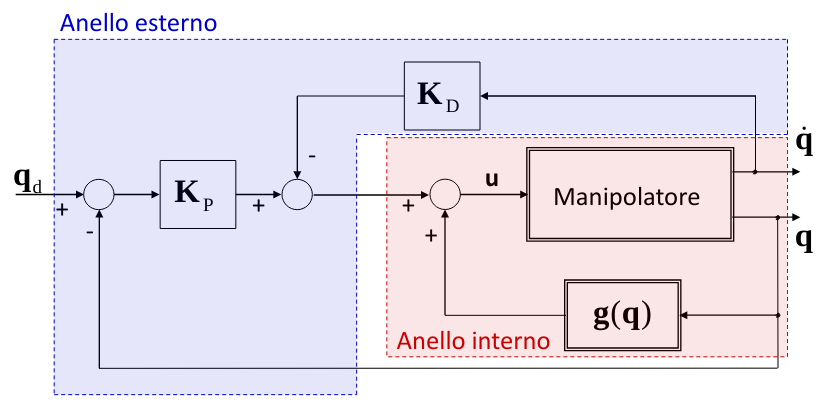
\includegraphics[width=0.6\linewidth]{images/centralized_control_pd_gravity_comp}
	\caption{Controllo PD con compensazione della gravità}
	\label{fig:centralizedcontrolpdgravitycomp}
\end{figure}
(notare che nel circuito non è presente $\dot{q}_d$: questo poichè essendo $q_d$ costante la sua derivata è nulla)

Analizzando il sistema risultante da (\ref{eq:pd_gravity_comp_dyn}), possiamo vedere che l'unico punto di equilibrio è dato da $q = q_d$:
\unboldmath
\begin{align*}
x \ \text{punto di equilibro} 
&\iff 
\dot{x} = \begin{pmatrix}\dot{q} \\ \ddot{q}\end{pmatrix} = 0
\stepcounter{equation}\tag{\theequation}\label{eq:pd_grav_comp_equil} \\
&\iff 
B(q)\cancelto{0}{\ddot{q}} + C(q, \dot{q})\cancelto{0}{\dot{q}} + F_v\cancelto{0}{\dot{q}} = K_P(q_d - q) - K_D\cancelto{0}{\dot{q}} \\
&\iff
0 = K_P(q_d - q) \\
&\iff
q = q_d
\end{align*}

Ovvero proprio quello che volevamo: stabilità in una postura costante $\mathbf{q}_d$.\\
Per fare un esempio, immagina il robot in figura \ref{fig:centralizedcontrolpdgravitycompexample}: il motori dovranno applicare delle coppie (i quali valori dipendono dal valore di $\mathbf{u}$ mostrato prima) per far rimanere il braccio in questa posizione statica.

\begin{figure}[H]
	\centering
	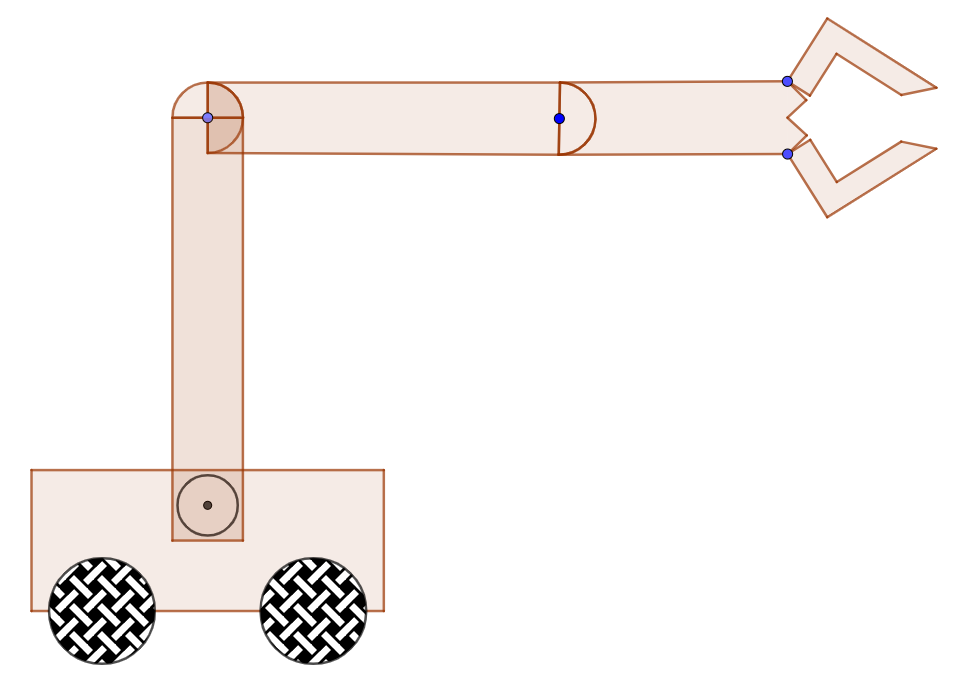
\includegraphics[width=0.5\linewidth]{images/centralized_control_pd_gravity_comp_example}
	\caption{Esempio di compensazione gravità}
	\label{fig:centralizedcontrolpdgravitycompexample}
\end{figure}




\vspace{20pt}
\subsubsection{Dimostrazione stabilità}
\boldmath
Per dimostrare le caratteristiche di stabilità del punto di equilibrio corrispondente alla postura desiderata, è possibile applicare il \textbf{metodo diretto di Lyapunov}. Definiamo $e \triangleq q_d - q$ e consideriamo come funzione di Lyapunov:
$$
V(\dot{q}, e) = \frac{1}{2}\dot{q}^TB(q)\dot{q} + \frac{1}{2}e^TK_Pe > 0    \qquad \forall q,e\neq0
$$
Dove possiamo interpretare il primo termine come l’energia cinetica del sistema ed il secondo come l’energia potenziale immagazzinata grazie alle rigidezze equivalenti date dai guadagni delle retroazioni delle posizioni ai giunti.

In questa funzione è stato scelto come stato del sistema il vettore $(e, \ \dot{q})^T$ che, dal punto di vista dell'equilibro, è equivalente a quanto usato in (\ref{eq:pd_grav_comp_equil}):
\begin{gather*}
\gamma \triangleq \begin{pmatrix}e \\ \dot{q}\end{pmatrix} = \begin{pmatrix}q - q_d \\ \dot{q}\end{pmatrix}
\implies 
\dot{\gamma} = \begin{pmatrix}\dot{e} \\ \ddot{q}\end{pmatrix} = \begin{pmatrix}\dot{q} - \cancelto{0}{\dot{q}_d} \\ \ddot{q}\end{pmatrix} = \begin{pmatrix}\dot{q} \\ \ddot{q}\end{pmatrix}
\end{gather*}



Ora passiamo allo studio del segno di $V$ lungo le traiettorie del sistema (come è richiesto dal metodo di Lyapunov). Derivando (ricordando che $\dot{q}_d = 0$, essendo $q_d$ costante), otteniamo:
$$
\dot{V} = \dot{q}^TB(q)\ddot{q} + \frac{1}{2}\dot{q}\dot{B}(q)\dot{q} - \dot{q}^TK_Pe
$$
procediamo sostituendo a $B(q)\ddot{q}$ la forma di esso fornita da (\ref{eq:pd_gravity_comp_dyn}) (ricordando la definizione di $e \triangleq q_d - q$):
\begin{gather*}
	B(q)\ddot{q} + C(q, \dot{q})\dot{q} + F_v\dot{q} = K_Pe - K_D\dot{q} \\
	\Updownarrow \\
	B(q)\ddot{q} = -C(q, \dot{q})\dot{q} - F_v\dot{q} + K_Pe - K_D\dot{q} \\
	\Downarrow \\
	\dot{V} = \dot{q}^T( -C(q, \dot{q})\dot{q} - F_v\dot{q} + \cancel{K_Pe} - K_D\dot{q} ) + \frac{1}{2}\dot{q}\dot{B}(q)\dot{q} - \dot{q}^T \cancel{K_Pe}
\end{gather*}

Raccogliendo i termini rimasti si ha
$$
\dot{V} = \frac{1}{2} \dot{q}^T ( \cancelto{0}{ \dot{B}(q) - 2C(q, \dot{q}) })\dot{q} - \dot{q}^T (F_v + K_D)\dot{q}
$$
dove la cancellazione a 0 è fatta grazie alla \textit{null-property} di quella differenza (si può dimostrare dalle equazioni della dinamica).

Allora:
$$
\dot{V} = - \dot{q}^T (F_v + K_D)\dot{q}
$$
che risulta essere \textbf{semi-definita negativa}. È solo \textbf{semi}-definita poichè è presente solo $\dot{q}$: $\dot{V} = 0$ per $\dot{q} = 0$ ma per qualsiasi $e$.

Possiamo però ora osservare che comunque $\dot{V} = 0 \iff \dot{q} = 0$, e di conseguenza anche $\ddot{q} = 0$. Ricordando da (\ref{eq:pd_grav_comp_equil}) che $(\dot{q}, \ddot{q}) = (0,0)$ è la condizione di equilibrio, possiaom dire che $\dot{V}$ si annulla solo per l'unico punto di equilibrio del sistema.
Dal teorema di \textit{La Salle-Krasowski} risulta pertanto globalmente asintoticamente stabile, come desiderato.
\unboldmath

\vspace{15pt}
\begin{addendum}
\textbf{Thm.} La Salle-Krasowski

Supponi che un sistema dinamico sia rappresentato da $\dot{\mathbf{x}}=f(\mathbf{x})$, dove $\mathbf{x}$ è il vettore dello stato e $f(\mathbf{0})=0$.\\
Se prendiamo una funzione $V$ tale che:
$$
\begin{cases}
	V(\mathbf{x}) > 0 \\
	\dot{V(\mathbf{x})} \leq 0
\end{cases}
$$
(i.e. $V$ positiva e $\dot{V}$ semi-definita negativa), \textbf{ma}
$$
\dot{V}(\mathbf{x}) = 0 \iff \mathbf{x} = 0
$$
allora abbiamo che l'\textbf{origine} $\mathbf{x} = 0$ è \textbf{asintoticamente stabile}.
\end{addendum}










\section{Controllo nello spazio operazionale}

